%
% modulation.tex
%
% (c) 2020 Prof Dr Andreas Müller, Hochschule Rapperswil
%
\subsection{Modulation zweidimensionaler Signale
\label{subsection:modulation}}
Wir streben jetzt an, ein zweidimensionales Signal
\[
\vec{v}(t)
=
\begin{pmatrix}I(t)\\Q(t)\end{pmatrix}
\]
drahtlos zu übertragen und müssen zu diesem Zweck ein geeignetes
Modulationsverfahren finden.

\begin{figure}
\centering
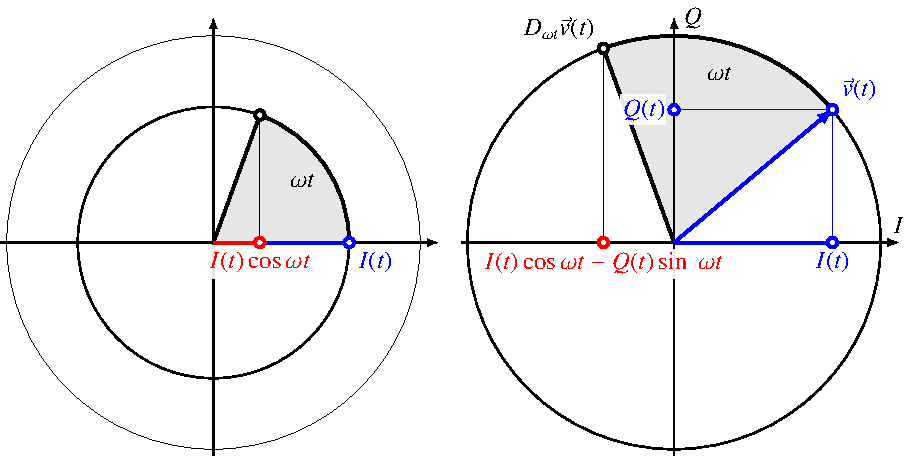
\includegraphics{applications/qam/images/icos.pdf}
\caption{Modulation des Signals $I(t)$ als Drehung um den Winkel $\omega t$
auf einem Kreis mit Radius $I(t)$.
\label{qam:figure:icos}}
\end{figure}
Mit nur dem einen Signal $I(t)$ haben wir $I(t)\cos\omega t$ als moduliertes
Signal gewählt.
Geometrisch können wir das auf einem Kreis mit Radius $I(t)$ als Drehung
um den Winkel $\omega t$ mit anschliessender Projektion auf die horizontale
Achse verstehen (Abbildung~\ref{qam:figure:icos} links).

Es ist daher naheliegend, für die Modulation des zweidimensionalen Signals
ebenfalls eine Drehung um den Winkel $\omega t$ zu verwenden.
Der Vektor $\vec{v}(t)$ wird in der $I$-$Q$-Ebene gedreht wie in
Abbildung~\ref{qam:figure:icos} rechts gezeigt.
Dazu kann eine Drehmatrix $D_{\omega t}$ verwendet werden.
Wir berechnen
\begin{equation}
D_{\omega t}
\vec{v}(t)
=
\begin{pmatrix}
\cos\omega t & -\sin\omega t\\
\sin\omega t &\phantom{-}\cos\omega t
\end{pmatrix}
\begin{pmatrix}I(t)\\Q(t)\end{pmatrix}
=
\begin{pmatrix}
I(t)\cos\omega t - Q(t) \sin\omega t\\
I(t)\sin\omega t + Q(t) \cos\omega t
\end{pmatrix}
=
\begin{pmatrix}
s(t)\\c(t)
\end{pmatrix}
\label{qam:eqn:modulation}
\end{equation}
Das zweite Signal $Q(t)$ modulieren wir also statt mit $\cos\omega t$ 
mit der Funktion $-\sin\omega t$.
Natürlich können wir aus den beiden Funktionen $I(t)\cos\omega t$ und
$-Q(t)\sin\omega t$ auch die Funktionen $I(t)$ und $Q(t)$ zurückgewinnen,
das reicht aber nicht.
Dazu brauchen wir nämlich $I(t)\cos\omega t$ und $-Q(t)\sin\omega t$
unabhängig voneinander, wir brauchen also zwei unabhängig Übertragungskanäle
für die beiden Signale, was wir vermeiden wollen.

\begin{figure}
\centering
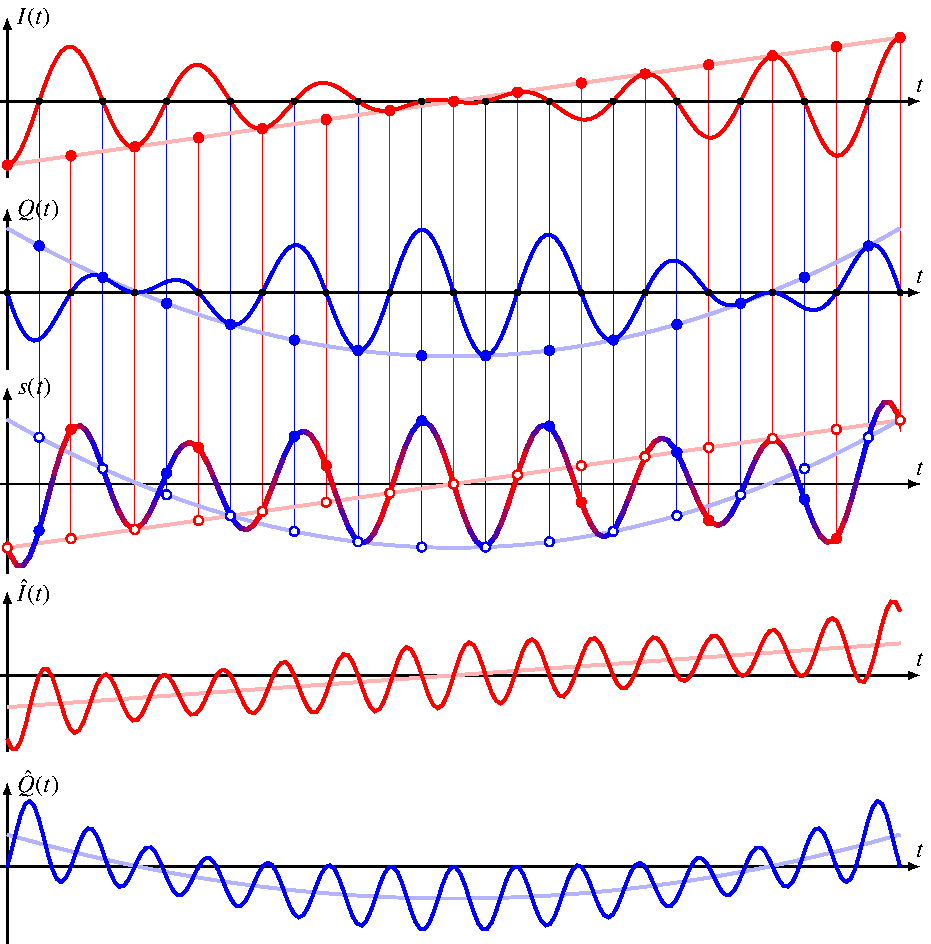
\includegraphics{applications/qam/images/sep.pdf}
\caption{Rekonstruktion der Signale $I(t)$ und $Q(t)$ (oberste zwei Graphen)
aus der Summe $s(t) = I(t)\cos\omega t - Q(t)\sin\omega t$ (Mitte).
Die Nullstellen von $\cos\omega t$ sind durch feine blaue Linien 
dargestellt, die Nullstellen von $\sin\omega t$ durch feine rote Linien.
Der Graph von $s(t)$ ist jeweils mit der Farbe eingefärbt, die den
dominanten Beitrag repräsentiert.
Blaue Segmente im Graphen von $s(t)$ bedeuten, dass vor allem der Wert
von $Q(t)$ zum Wert beiträgt, dies geschieht in der Umgebung von
Nullstellen von $\cos\omega t$, in den roten Segmenten ist es der Wert von
$I(t)$, welcher dominiert während $\sin\omega t$ eine Nullstelle durchläuft.
Fette Punkte auf dem Graphen von $s(t)$ markieren Punkte bei den
genannten Nullstellen.
Die leeren Punkte sind Werte von $s(t)$, die um das Vorzeichen des
Trägeres korrigiert wurden, sie liegen genau auf dem Graphen der
ursprünglichen Signale $I(t)$ und $Q(t)$.
Die untersten zwei Graphen zeigen die rekonstruierten Signale
$\hat{I}(t)=s(t) \cos\omega t$ und $\hat{Q}(t) = -s(t) \sin\omega t$, 
welche in Abschnitt~\ref{subsection:demodulation} erklärt werden.
\label{figure:qam:sep}}
\end{figure}

Einzelne Werte der Funktionen $I(t)$ und $Q(t)$ können aber aus der Summe
\[
s(t)
=
I(t)\cos\omega t - Q(t)\sin\omega t
\]
rekonstruiert werden.
An den Stellen $t = k\pi/\omega$ für $k\in\mathbb Z$ verschwindet
der Faktor $\sin\omega t$,
so dass an diesen Stellen der zweite Summand in $s(t)$ wegfällt.
Ebenso wird der erste Summand an den Stellen
$t = (k+\frac12)\pi/\omega$ verschwinden.
Dieser Sachverhalt ist in Abbildung~\ref{figure:qam:sep} dargestellt.
Es ist also
\[
s\biggl(k\cdot \frac{\pi}{2\omega}\biggr)
=
\begin{cases}
I(k\cdot \frac{\pi}{2\omega})\cdot(-1)^{\frac{k}2}
&\qquad \text{$k$ gerade,}\\[5pt]
Q(k\cdot \frac{\pi}{2\omega})\cdot(-1)^{\frac{k-1}2}
&\qquad \text{$k$ ungerade.}
\end{cases}
\]
Zu Zeitpunkten, die Vielfache von $\pi/2\omega$ sind, kann man also aus
$s(t)$ die Werte von $I(t)$ und $Q(t)$ ablesen.
Tatsächlich lernt man im Fach {\em Signale und Systeme}, dass man daraus
die Funktionen $I(t)$ und $Q(t)$ rekonstruieren kann, wenn sie keine
Frequenzkomponenten grösser als die Trägerfrequenz haben.
Die Summe $s(t)$ ist also etwas, was man potentiell drahtlos übermitteln
kann, und woraus man die Komponenten $I(t)$ und $Q(t)$ zurückgewinnen kann.
Man nennt dieses Modulationsverfahren {\em Quadratur-Amplituden-Modulation}.

Da wir über das nötige signaltheoretische Wissen noch nicht verfügen,
müssen wir eine alternative, geometrische Methode suchen, wie wir
aus $s(t)$ die Komponenten $I(t)$ und $Q(t)$ wiedergewinnen können.
Das modulierte Signal $s(t)$ ist also nichts anderes als eine
Komponente eines Vektors, der entsteht indem $\vec{v}(t)$ mit sehr grosser
Winkelgeschwindigkeit $\omega$ um den Ursprung gedreht wird.
Wir sind aber insofern nicht weiter, dass wir $I(t)$ und $Q(t)$ noch nicht
rekonstruieren können.



